\section{Lenstra's jewellery}
In the third part, we'll show how to lift the ring structure on~$\mathrm{M}_{n}(A)$ to~$\Lambda_{n}(A)$, and onwards to~$\Lambda(A)$. Patient readers \sout{will} might even get a present, depending on their linguistic background.

\subsection{Idea}

\begin{wrapfigure}[13]{r}{.35\textwidth}
  \centering
  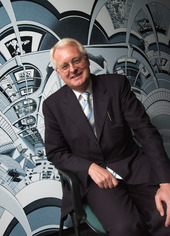
\includegraphics[width=.3\textwidth]{playing-witt-rings/lenstra}
  \caption{Hendrik Lenstra}
\end{wrapfigure}

Remember that~$\mathrm{M}_{n}(A)=\langle {1-aT  \vert  a \in A} \rangle$. If~$A$ were an algebraically closed field, every monic polynomial over~$A$ would split into products of linear factors, thus showing that~$\Lambda_{n}(A)=\mathrm{M}_{n}(A)$. This would make our life easy, since we just adorned~$\mathrm{M}_{n}(A)$ with a ring structure. In general, this isn't the case, but we'll show that there exists a ring~$\overline{A}$ containing~$A$ for which the property holds. Equipped with this bigger ring, we'll want to conclude that~$\Lambda_{n}(A) \subset \Lambda_{n}(\overline{A})$, so that the ring structure we put on~$\mathrm{M}_{n}(\overline{A})=\Lambda_{n}(\overline{A})$ gets inherited by~$\Lambda_{n}(A)$. From then on, it'll be easy to pass over to~$\Lambda(A)$.

\subsection{Close up}

Starting with a commutative ring~$A$, look at the set of all monic polynomials of strictly positive degree, say~$M$. We now define a new~$A$-algebra~$A'$ as the tensor product over all these polynomials of~$A[X_{f}]/(f)$. By direct limit construction, this tensor product is an algebra (check out Chapter~$2$, Exercise~$23$ in \cite{atiyah-macdonald} if you don't know this stuff). It's easy to convince yourself that
\begin{equation}
  A'=A[X_{f}:f \in M]/(f(X_{f}):f \in M).
\end{equation}
You should think of~$A'$ as the algebra we get by adjoining a root, $\alpha_{f}$, which is the image of~$X_{f}$ in~$A'$, for all polynomials in~$M$. We can take as a basis for the~$A$-module~$A'$ all `monomials'
\begin{equation}
  \prod_{f \in M} \alpha_{f}^{i(f)}, \quad\text{with } 0\leq i(f) < \deg(f), 
\end{equation}
with all but finitely many of the~$\alpha_{f}$'s equal to~$0$. This basis includes~$\overline{1_{A}}$, which makes the natural map from~$A$ to~$A'$ injective, showing that~$A \subset A'$. Denoting~$A$ by~$A^{(0)}$,~$A'$ by~$A^{(1)}$, we can keep on repeating the process to get~$A$-algebras~$A^{(n)}$. The algebra we're looking for is
\begin{equation}
  \overline{A}=\varinjlim_{n} A^{(n)}. 
\end{equation}
Direct limits exist for algebras over a ring (again, see the exercises in~\cite{atiyah-macdonald}), and every polynomial in~$\overline{A}[X]$ splits over some~$A^{(n)}$, and thus over~$\overline{A}$. This is exactly the structure we'd like to have, for which~$\mathrm{M}_{n}(\overline{A})=\Lambda_{n}(\overline{A})$.

\subsection{Ring structure on~$\Lambda_{n}(A)$}

To make~$\Lambda_{n}(A)$ into a subring of~$\Lambda_{n}(\overline{A})$, it has to be closed under multiplication. To prove this, we'll need a small lemma, which will also come in handy while proving functoriality of the~$\Lambda_{n}$'s.

\begin{lemma}
  Suppose~$A \subset B$ commutative rings,~$u,v \in \Lambda_{n}(A)$, with~$u, v \in \mathrm{M}_{n}(B)$. Then~$u*_{B}v = u*_{\overline{A}}v \in \Lambda_{n}(A)$.

  \begin{proof}
    Extending scalars, define~$C=B \otimes_{A} \overline{A}$. From the  previous paragraph, we know that, as an~$A$-module,~$\overline{A}=A \cdot 1 + \bigoplus_{i \in I} Ae_{i}$. This implies that~$C=B \cdot 1 + \bigoplus_{i \in I} Be_{i}$. Thus~$\overline{A}, B \subset C$ and inside~$C$ we have~$B \cap \overline{A}=A$. Since~$*$ is functorial in~$A$, and~$B \subset C$,~$u*_{B}v=u*_{C} v=u  *_{\overline{A}}  v$, and this unique element lies in~$\Lambda_{n}(A)$, by passing to the~$\Lambda_{n}$ in the above cap-identity.
  \end{proof}
\end{lemma}

If we take as~$B$ the ring~$\overline{A}$ itself, then~$\Lambda_{n}(A)$ is a subring of~$\Lambda_{n}(\overline{A})$, which we hoped for all along. More than this,~$\Lambda_{n}$ is functorial in~$A$. To see this, suppose~$f$ is a ring morphism, and look at the induced map~$\Lambda_{n}(f)$. We have to prove that the image of~$u  *_{A}  v$ is equal to~$\Lambda_{n}(f)(u)  *_{B}  \Lambda_{n}(f)(v)$. Since~$u$ and~$v$ are in~$\Lambda_{n}(A)$, and thus in~$\mathrm{M}_{n}(\overline{A})$, their images~$\Lambda_{n}(f)(u)$ and~$\Lambda_{n}(f)(v)$ are in~$\mathrm{M}_{n}(B \otimes_{A} \overline{A})$. By again applying the lemma for~$B \subset B \otimes_{A} \overline{A}$, the product of these images can be computed in~$\mathrm{M}_{n}(B \otimes_{A} \overline{A})$. From a previous post we know that~$\mathrm{M}_{n}$ is a functor, which means that this product is equal to the image of~$u  *_{A}  v$, showing that~$\Lambda_{n}(f)$ is a ring morphism.

\subsection{At last,~$\Lambda(A)$!}

We now know that each~$\Lambda_{n}$ is an endofunctor in the category~$\textsf{CRing}$, and that the maps~$\Lambda_{n+1} \to \Lambda_{n}$ are natural transformations (again, this can easily be checked). This means we can take the projective limit of the functors~$\Lambda_{n}$,
\begin{equation}
  \varprojlim_{n} \Lambda_{n} = \Lambda,
\end{equation}
which supplies~$\Lambda(A)$ with a ring structure, in a nice functorial way, satisfying all our needs. Of course, nothing here shows that this structure is unique. This can be proven by some abstract nonsense, and a dash of topology, for which I refer you to Lenstra's paper. If I feel like it, I'll add a last post next week, describing how to pass from~$\Lambda(A)$ to the Witt ring one usually finds in the literature,~$\mathrm{W}(A)$. I might throw in some actual computations to show you that~$\Lambda(A)$ isn't that hard to work with, just a little messy.

For those who stuck with me, here's a little reward: a documentary about the life of Hendrik Lenstra, \href{http://www.human.nl/programma-35637-magie-van-de-wetenschap}{De dingen die je niet begrijpt}. Hope you know some Dutch!
